\section{Durchführung}
\label{sec:Durchführung}

\subsection{Aufbau}
Der Aufbau der Messapparatur ist in Abb. \ref{fig:Aufbau} zu sehen.
\begin{figure}
    \centering
    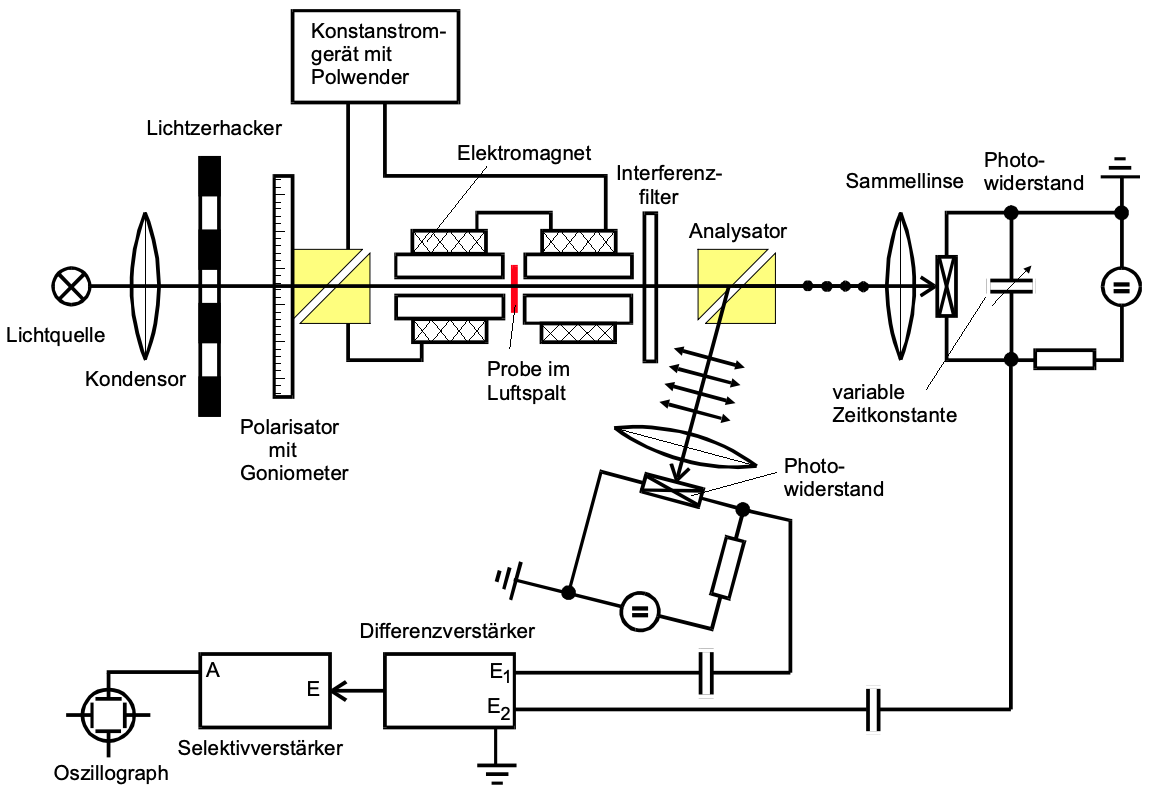
\includegraphics[width=15cm]{fotos/Aufbau.png}
    \caption{Der schematische Aufbau der Messapparatur. \cite{V46}}
    \label{fig:Aufbau}
\end{figure}
Das Gleichlicht der Halogenlampe wird durch einen Lichtzerhacker in Impulse zerhackt, damit mit einer Wechsellichtmethode gearbeitet werden kann. Das Licht wird außerdem durch einen Interferenzfilter monochromatisiert und durch ein Glan-Thompson-Prisma linear polarisiert. Die Probe befindet sich im Luftspalt eines Elektromagneten, der von einem Konstantstromgerät gespeist wird, das eine Polwendevorrichtung besitzt (um den Drehwinkel zu verdoppeln). Das Glan-Thompson-Prisma teilt den Lichtstrahl in zwei Strahlbündel, die senkrecht zueinander polarisiert sind. Die Lichtintensität wird jeweils mit einem Photowiderstand gemessen, indem eine Gleichspannung durchgeschickt und der Spannungsabfall gemessen wird (Innenwiderstand ist proportional zur Intensität). Mithilfe eines Differenzverstärkers, der an einen Oszillographen angeschlossen ist, kann festgestellt werden, ob die beiden Signalspannungen gleich sind.

\subsection{Justierung}
Die Messapparatur wird mit sichtbarem Licht justiert. Dazu werden Probe und Interferenzfilter entfernt.
Zunächst werden die Prismen so ausgerichtet, dass das Licht senkrecht zu ihrer Oberfläche einfällt. Durch Drehen des Analysatorprismas um seine vertikale Achse wird die Lichtintensität des durchgehenden Strahls eliminiert.
Anschließend wird das Licht auf die lichtempfindlichen Flächen der Photowiderstände abgebildet.
Es wird eine Wechsellichtfrequenz von einigen Hundert Hertz eingestellt. Die Mittenfrequenz des Selektivverstärkers wird auf diese Frequenz eingeregelt und der Gütefaktor auf seinen Maximalwert (Q = 100).
Probe und Interferenzfilter werden eingesetzt und alles wird verbunden. Zuletzt wird überprüft, ob die Signalamplitude durch Drehen des Polarisators auf nahezu Null gebracht werden kann.

\subsection{Messung}
Zuerst wird mithilfe einer Hallsonde die Kraftflussdichte in Richtung des einfallenden Lichts in der Nähe des Luftspalts bei maximalem Feldstrom gemessen.

Als nächstes wird die Faraday-Rotation an zwei n-dotierten GaAs-Proben für verschiedene Wellenlängen im nahen Infrarot gemessen. Dazu werden neun verschiedene Interferenzfilter, die eine Wellenlänge filtern, verwendet.
Die Drehung der Polarisationsebene (Faraday-Rotation) wird folgendermaßen gemessen: bei maximalem Feld wird die gleiche Lichtintensität für beide Strahlen eingestellt (Spannung Null am Differenzverstärker). Das wird erreicht, indem abwechselnd das erste Glan-Thompson-Prisma um seine Längsachse gedreht (die Winkelstellung wird am fest mit dem Prisma verbundenen Goniometer abgelesen) und die Zeitkonstante der beiden Photowiderstände aneinander angepasst wird. Anschließend wird das Feld umgepolt und es wird wieder auf Signalspannung Null abgeglichen. Der zweite Drehwinkel kann am Goniometer abgelesen werden. Die Drehung der Polarisationsebene ist dann die Hälfte der Differenz der beiden Drehwinkel.

Zuletzt wird die gleiche Messung für hochreines GaAs wiederholt.